\documentclass[]{elsarticle} %review=doublespace preprint=single 5p=2 column
%%% Begin My package additions %%%%%%%%%%%%%%%%%%%
\usepackage[hyphens]{url}

  \journal{Geographical Analysis} % Sets Journal name


\usepackage{lineno} % add
\providecommand{\tightlist}{%
  \setlength{\itemsep}{0pt}\setlength{\parskip}{0pt}}

\usepackage{graphicx}
\usepackage{booktabs} % book-quality tables
%%%%%%%%%%%%%%%% end my additions to header

\usepackage[T1]{fontenc}
\usepackage{lmodern}
\usepackage{amssymb,amsmath}
\usepackage{ifxetex,ifluatex}
\usepackage{fixltx2e} % provides \textsubscript
% use upquote if available, for straight quotes in verbatim environments
\IfFileExists{upquote.sty}{\usepackage{upquote}}{}
\ifnum 0\ifxetex 1\fi\ifluatex 1\fi=0 % if pdftex
  \usepackage[utf8]{inputenc}
\else % if luatex or xelatex
  \usepackage{fontspec}
  \ifxetex
    \usepackage{xltxtra,xunicode}
  \fi
  \defaultfontfeatures{Mapping=tex-text,Scale=MatchLowercase}
  \newcommand{\euro}{€}
\fi
% use microtype if available
\IfFileExists{microtype.sty}{\usepackage{microtype}}{}
\bibliographystyle{elsarticle-harv}
\usepackage{graphicx}
% We will generate all images so they have a width \maxwidth. This means
% that they will get their normal width if they fit onto the page, but
% are scaled down if they would overflow the margins.
\makeatletter
\def\maxwidth{\ifdim\Gin@nat@width>\linewidth\linewidth
\else\Gin@nat@width\fi}
\makeatother
\let\Oldincludegraphics\includegraphics
\renewcommand{\includegraphics}[1]{\Oldincludegraphics[width=\maxwidth]{#1}}
\ifxetex
  \usepackage[setpagesize=false, % page size defined by xetex
              unicode=false, % unicode breaks when used with xetex
              xetex]{hyperref}
\else
  \usepackage[unicode=true]{hyperref}
\fi
\hypersetup{breaklinks=true,
            bookmarks=true,
            pdfauthor={},
            pdftitle={A spatial analysis of the environmental correlates of COVID-19 incidence in Spain},
            colorlinks=false,
            urlcolor=blue,
            linkcolor=magenta,
            pdfborder={0 0 0}}
\urlstyle{same}  % don't use monospace font for urls

\setcounter{secnumdepth}{0}
% Pandoc toggle for numbering sections (defaults to be off)
\setcounter{secnumdepth}{0}


% Pandoc header
\usepackage{booktabs}
\usepackage{longtable}
\usepackage{array}
\usepackage{multirow}
\usepackage{wrapfig}
\usepackage{float}
\usepackage{colortbl}
\usepackage{pdflscape}
\usepackage{tabu}
\usepackage{threeparttable}
\usepackage{threeparttablex}
\usepackage[normalem]{ulem}
\usepackage{makecell}
\usepackage{xcolor}



\begin{document}
\begin{frontmatter}

  \title{A spatial analysis of the environmental correlates of COVID-19 incidence
in Spain}
    \author[McMaster University]{Antonio Paez\corref{1}}
   \ead{paezha@mcmaster.ca} 
    \author[Universidad Politecnica de Cartagena]{Fernando A. Lopez}
   \ead{fernando.lopez@upct.es} 
    \author[Departamento de Economia]{Tatiane Menezes}
   \ead{tatiane.menezes@ufpe.br} 
    \author[Nucleo de Pesquisa]{Renata Cavalcanti}
   \ead{renata.vcsantos@gmail.com} 
    \author[Nucleo de Pesquisa]{Maira Galdino da Rocha Pitta}
   \ead{mgrpitta@ufpe.br} 
      \address[McMaster University]{School of Geography and Earth Sciences, McMaster University, 1281 Main
St W, Hamilton, ON, L8S 4K1, Canada}
    \address[Universidad Politecnica de Cartagena]{Departamento de Metodos Cuantitativos, Ciencias Juridicas, y Lenguas
Modernas, Universidad Politecnica de Cartagena, Calle Real Numero 3,
30201, Cartagena, Murcia, Spain}
    \address[Departamento de Economia]{Departamento de Economia, Universidade Federal de Pernambuco, Av dos
Economistas, s/n - Cidade Universitária, Recife - PE, 50670-901, Brasil}
    \address[Nucleo de Pesquisa]{Núcleo de Pesquisa em Inovação Terapêutica NUPIT / UFPE, Av.
Prof.~Moraes Rego, 1235 - Cidade Universitária, Recife, PE, CEP
50670-901, Brazil}
      \cortext[1]{Corresponding Author}
  
  \begin{abstract}
  Spreading with astonishing speed, the novel SARS-CoV2 has swept the
  globe, causing enormous stress to health systems and prompting social
  distance guidelines and mandates to arrest its progress. While there is
  encouraging evidence that early public health interventions have slowed
  the spread of the virus, this has come at a high cost as the global
  economy is brought to its knees. How and when to ease restrictions to
  movement hinges in part on the question whether SARS-CoV2 will display
  seasonality associated with variations in temperature, humidity, and
  hours of sunshine. In this research, we address this question by means
  of a spatial analysis of the incidence of COVID-19 in the provinces in
  Spain. Use of a spatial Seemingly Unrelated Regressions (SUR) approach
  allows us to model the incidence of reported cases of the disease per
  100,000 population, as a function of temperature and humidity, while
  controlling for GDP per capita, population density, percentage of older
  adults in the population, and presence of mass transit systems. An
  interesting aspect of the spatial SUR approach is that it models
  incidence as a contagion process. Our results indicate that incidence of
  the disease is lower at higher temperatures and higher levels of
  humidity, although coefficients for this variable are significant only
  in some equations. Sunshine, in contrast, displays a positive
  association with incidence of the disease. Our control variables also
  yield interesting insights. Higher incidence is associated with higher
  GDP per capita and presence of mass transit systems in the province; in
  contrast, population density and percentage of older adults display
  negative associations with incidence of COVID-19.
  \end{abstract}
  
 \end{frontmatter}

\hypertarget{introduction}{%
\section{Introduction}\label{introduction}}

From a small outbreak linked to a live animal market at the end of 2019
to a global pandemic in a matter of weeks, the SARS-CoV2 virus has
threatened to overrun health systems the world over. In efforts to
contain the spread, numerous governments in many nations and regions
have either recommended or mandated social distancing measures, and as
of this writing, millions of people in five continents shelter in place.
There are encouraging signs that these measures have arrested the spread
of the virus where they have been implemented, and have thus helped to
keep a bad situation from becoming even worse (e.g., 2020). However,
this has come at a high cost, and the consequences for all spheres of
the economy, social, and cultural life have been dire (e.g., Fernandes,
2020; Luo and Tsang, 2020). As a result, there is a sense of urgency to
anticipate the progression of the pandemic, in order to plan for
progressive lifting of restrictions to movement and social contact
(e.g., Kissler et al., 2020). Needless to say, this has become a
delicate, and politically charged, balancing act between public health
and the economy (Gong et al., 2020).

A salient question in the debate on how and when to ease social
distancing measures is whether the virus will display seasonal
variations. Earlier, diverse studies have shown the effect of
temperature and humidity on the incidence of influenza (e.g., Mäkainen
et al., 2009; Jaakkola et al., 2014; Kudo et al., 2019). Jaakkola et
al.~(2014), for example, found that a decrease of temperature and
absolute humidity precedes the onset of symptoms of influenza A and B
viruses by 3 days in places where the temperature is low. After the
2002-2004 outbreak of SARS, researchers also began to investigate the
relationship between these factors and SARS-CoV. In this way, Casanova
et al.~(2010) used two surrogates, namely the gastroenteritis (TGEV) and
mouse hepatitis viruses (MHV), to find that virus inactivation was more
rapid at temperatures of 20C than 4C, and at 40C than 20C; in terms of
humidity, these researchers reported that survival of the virus was
lower at moderate relative humidity levels. In a similar vein, but
working directly with SARS-CoV, Chan et al.~(2011) found that viability
of the virus was lost at temperatures higher than 38C and relative
humidity superior to 95\%.

While existing research on similar pathogens suggests that SARS-CoV is
more stable and potentially easier to transmit in conditions of low
temperature and low humidity, it is far from certain that this will also
be the case with the novel SARS-CoV2. If such is the case, there is the
possibility of easing restrictions to social contact as the weather
warms; however, weeks or possibly months of costly measures could become
undone if not, and the restrictions are lifted prematurely. Not
surprisingly, given the stakes involved, this issue has already
triggered a lively debate.

Some of what is thought about the possible seasonality of COVID-19 is
based on analogies to the patterns of other known respiratory viruses.
However, de Ángel Solá et al.~(2020) note that ``not all seasonal
respiratory viruses experience the same spatiotemporal patterns''
(section 4). This urges caution when extrapolating from known viruses,
and indeed, the evidence in this respect is inconclusive. At a global
scale, de Ángel Solá et al.~(2020) see less risk in the Caribean Basin;
however, Coelho et al.~(Coelho et al., 2020) warn that at least during
the exponential phase, expansion of the virus is not driven by climate.
Similarly, whereas Araujo and Naimi (2020) argue that spread of
SARS-CoV2 will likely be constrained by climate, Harbert et al.~(2020)
remain unconvinced that spatial modelling can currently discriminate the
distribution of the disease on the basis of climate, at least in the
United States. Yao et al.~(2020), examined data from China and came to
the conclusion that neither temperature nor ultraviolet indices had an
association with transmission of COVID-19. This is despite previous
research that has linked less exposure to UVB radiation to higher
prevalence and severity of acute respiratory tract infections
(Zittermann et al.~2016; Dąbrowska-Leonik et al.~2018; Dinlen et
al.~2016; Mathyssen et al.~2017; Esposito and Lelii 2015; Jat 2017;
Moriyama, Hugentobler, and Iwasaki 2020). To further complicate matters,
much of the relevant work has yet to be peer-reviewed and therefore is
open to change (see for example the challenge of Harbert et al. (2020)
to Araujo and Naimi (2020)). In the United States, the National Academy
of Sciences, Engineering, and Medicine was engaged by the Office of the
Executive for guidance on this matter (see National Academies of
Sciences, Engineering and Medicine, 2020). Their conclusion summarizes
the situation well (see p.~6): ``Some limited data support a potential
waning of cases in warmer and more humid seasons, yet none are without
major limitations\ldots Additional studies as the SARS-CoV-2 pandemic
unfolds could shed more light on the effects of climate on
transmission.''

With the above considerations in mind, our objective with this paper is
to contribute to the knowledge basis regarding the spread of COVID-19
and the influence of environmental factors, particularly temperature,
humidity, and sunshine. We adopt a population health approach, and
report results from a spatial model of the incidence of COVID-19 in
fifty provinces in Spain, one of the countries hardest hit by the
pandemic. We combine data on reported cases of the disease with
metereological information, to create a spatio-temporal dataset covering
a period of 30 days. We then join this dataset with provincial-level
economic and demographic information to act as controls to our key
environmental variables. These data are analyzed using a spatial
Seemingly Unrelated Regressions (SUR) approach, which allows us to model
incidence of COVID-19 as a spatial contagion process.

The results provide evidence of the effect of temperature, humidity, and
sunshine on the incidence of COVID-19. The clearest result with respect
to these variables is a lower incidence of COVID-19 at higher
temperatures and levels of humidity, while the opposite happens with
respect to hours of sunshine. Our control variables also provide some
intriguing insights. Higher incidence is associated with higher GDP per
capita and presence of mass transit systems in the province; in
contrast, population density and percentage of older adults display
negative associations with incidence of COVID-19. The results of this
analysis provide support to the hypothesis of seasonality of the novel
SARS-CoV2, and should be of interest to public health officials and
policy makers grappling with the question of the trajectory of the
pandemic.

Please note that this paper is prepared as a reproducible research
document. The source R Markdown document, as well as all data and code
needed to reproduce/review/extend the analysis can be obtained from the
following repository:

https://github.com/paezha/covid19-environmental-correlates/tree/master/Environmental-Correlates-of-COVID19-Spain

\hypertarget{context-data-and-methods}{%
\section{Context, Data, and Methods}\label{context-data-and-methods}}

\hypertarget{covid-19-in-spain}{%
\subsection{Covid-19 in Spain}\label{covid-19-in-spain}}

The first reported case of COVID-19 in Spain was on January 31th, when a
German tourist in the Canary Islands tested positive for the virus.
However, it was still a few weeks before the first domestic case was
reported, on February 27th in Sevilla province (Andalusia). In a short
period of time, after this relatively slow start, the outbreak flared.
By March 11th the World Health Organization (WHO) declared COVID-19
officially a pandemic. This declaration marked a turning point for the
public in Spain too. As of March 13th, the number of cases of COVID-19
reported in Spain was 4,473, with a majority of cases (1,990)
concentrated in Madrid: these numbers were at the time the worst
outbreak in Europe, after Italy. In response to the situation, on March
13th the Spanish National Government declared a state of emergency, to
go into effect on Saturday March 14th. As part of the state of emergency
restrictions to most activities were imposed, with the exception of
essential services (e.g.~food, health) and some economic subsectors of
industry and construction. A few days later, on March 17th, Spain closed
its lands borders to allow entry only to returnee nationals and
permanent residents. The lockdown was further hardened between March
30th and April 12th (including the Easter weekend of April 10th-12th)
and during this period only essential activities were allowed. During
this period, there was a dramatic reduction in overall mobility, both
within provinces as between
\footnote{https://www.mitma.gob.es/ministerio/covid-19/evolucion-movilidad-big-data/movilidad-provincial}.

\hypertarget{selection-of-variables}{%
\subsection{Selection of Variables}\label{selection-of-variables}}

The global emergence of infectious diseases is mostly driven by
environmental, ecological, and socio-economic factors (Jones et al.,
2008). In the case of SARS-CoV2, the ecological factors include the
interaction between humans and wildlife. Once transmission of a disease
begins to happen between humans, socio-economic and environmental
factors become increasingly important. As noted in the introduction, the
focus of the paper is on environmental variables, namely temperature,
humidity, and sunshine. These variables have been implicated in the
viability and ease of transmission of similar viruses. In addition to
these variables, we also aim to use a set of controls, in the form of
specific socio-economic and demographic characteristics of each
province.

The first variable that we consider is GDP per capita. Much has been
said about globalization and the spread of infectious
disease\footnote{As the Globe and Mail, Canada's paper of record, put it in relation to the SARS outbreak in 2003: "Globalization means that if someone in China sneezes, someone in Toronto may one day catch a cold" (Editorial, March 28, 2003, p. A18)}.
The growth in global connections has presented a challenge to spatial
approaches in the initial stages of disease management, when its cause
may still be unclear (Zhou and Coleman, 2016). In reference to the
earlier outbreak of SARS, van Wagner (Van Wagner, 2008) remarks how
Toronto's status as a global city was a vulnerability. In our case, we
think of GDP per capita as a marker of a region's relative position in a
network of global cities, and their potential to be further ahead in the
trajectory of the pandemic. Furthermore, wealthier regions also tend to
concentrate more activities that produce non-traded goods, including
building and construction (Hallet, 2002). Therefore, it is possible that
wealthier regions remained relatively more active even during the
lockdown. On the other hand, it is also possible the less wealthy
regions have a higher proportion of workers in manual occupations that
cannot telework.

The percentaje of older adults (over 65) is the second variable that we
consider as a control. Early evidence suggest that the case rate
mortality is higher at older ages (e.g.~The Novel Coronavirus Pneumonia
Emergency Response Epidemiology Team, 2020). It is not clear that
presence of older adults necessarily translates into higher transmission
in the population. The public health tool of choice in containing the
spread of the disease has been social distancing. In this respect, the
evidence from the field of transportation is that older adults tend to
travel less frequently, for shorter distances, and have higher rates of
immobility (e.g., Roorda et al., 2010; Morency et al., 2011; Sikder and
Pinjari, 2012). In other words, older adults are, by preference or
necessity, already in a form of social isolation. Social distancing
during the pandemic may actually reinforce that condition for older
adults, as the analysis of age-structured social contact in India,
China, and Italy of Sing and Adhikari (2020) suggests. Accordingly, our
expectation is that in the provinces with higher proportions of older
adults will tend to have similarl levels of lower social contact,
particularly since age-structured social contact matrix in Spain is
similar to Italy (Prem et al., 2017).

The third population variable the we consider is population density,
since it directly affects the contact patterns and contact rates between
individuals in a population (Hu et al., 2013). The evidence available
suggests a positive relationship between the transmission of COVID-19
and population density (e.g.~cumulative incidence in urban areas like
NYC). For this reason, we anticipate a positive relationship between
population density and the incidence of the disease.

The last control variable is the presence of mass transit systems in a
province. Every province in Spain offers some form of public
transportation, however only five provinces have higher order systems of
mass mobility, namely Barcelona, Madrid, Sevilla, Valencia, and Bizkaia.
Public transportation has been hypothesized to relate to the spread of
contagious disease by some researchers using agent-based approaches
(Perez and Dragicevic, 2009; Wang et al., 2010), and while we find scant
evidence of a link in the literature, the idea is intuitively appealing.
After all, unlike the isolation that a car offers to travellers, most
mass transit system are cauldrons of social contact.

\hypertarget{data}{%
\subsection{Data}\label{data}}

Our dataset includes information about the daily number of cases of
COVID-19 reported in Spain at the provincial level (NUTIII in Eurostat
terminology) for the period between March 13th and April 11th,
inclusive. For our purposes, we consider positive cases reported, but
excluding symptomatic cases diagnosed by a doctor without a Polymerase
Chain Reaction (PCR) test. The Spanish National Government publishes
periodic updates at the regional level (NUTII) and the information is
also released at the provincial level as part of a collaborative project
by geovoluntarios.com\footnote{https://www.geovoluntarios.org/},
ProvidencialData19\footnote{https://www.datoscovid.es/pages/providencialdata19},
and ESRI España. This information is compiled from several sources,
mainly the official web pages of the Spanish regional goverments, as
documented in Centro de Datos
Covid-19\footnote{https://www.datoscovid.es/pages/sobre-la-iniciativa}.
In addition, we consider two sets of explanatory variables. The first
one, and the focus of this research, is set of two environmental
variables, namely temperature and humidity, which are collected from
official sources (i.g., \emph{AEMET}, the state meteorology agency, and
\emph{MAPA}, the ministry of agriculture, fisheries, and food). The
second set provides some relevant controls for multivariate analysis,
and refers to economic and demographic attributes of the province (also
collected from official sources, i.e., INE, the national statistics
institute). Table \ref{tab:descriptive-statistics} shows the descriptive
statistics and the provenance of the data.

The spatial and temporal coverage of the data is as follows. Our dataset
begins on March 13, which is the first date when every province had
reported at least one case of COVID-19, and continues until April 11,
for a period of 30 days. The unit of analysis is the province. Provinces
are the equivalent of states, and are embedded in Autonomous
Communities. As an example, Cataluña is an Autonomous Community and
consists of four provinces, namely Barcelona, Gerona, Lerida, and
Tarragona. The size of the provinces is relatively large, as seen in
Table \ref{tab:descriptive-statistics}. The smallest province is
\(1,978.12km^2\) (this is smaller than Rhode Island in the US) and the
largest province is \(21,767.93km^2\) (slightly smaller than New Jersey
in the US). While this is a relatively large degree of spatial
aggregation, reporting on COVID-19 is inconsistent at smaller
geographies, or cases are not reported at that level at all. The
analysis must therefore be considered ecological.

\begin{table}

\caption{\label{tab:descriptive-statistics}\label{tab:descriptive-statistics} Descriptive statistics}
\centering
\resizebox{\linewidth}{!}{
\begin{tabular}[t]{l>{\raggedright\arraybackslash}p{15em}rrrr>{\raggedright\arraybackslash}p{5em}}
\toprule
Variable & Note & Min & Mean & Max & SD & Source\\
\midrule
\rowcolor{gray!6}  COVID-19 Incidence & Incidence in reported cases of SARS-19 per 100,000 people & 0.38 & 153.61 & 1149.36 & 186.23 & ProvidencialData19\\
Area & Area of province in sq.km & 1978.12 & 10118.79 & 21767.93 & 4.77 & INE\\
\rowcolor{gray!6}  GDPpc & GDP per capita in €1,000s & 16.67 & 22.51 & 36.00 & 4805.98 & INE\\
Older & Percentage of people aged 65 and older in the province & 15.16 & 21.03 & 31.36 & 3.95 & INE\\
\rowcolor{gray!6}  Population Density & Population density in the province in people per sq.km & 8.60 & 140.04 & 829.76 & 181.25 & INE\\
\addlinespace
Mean Temperature & Mean temperature in province by date, in C & 1.00 & 12.18 & 23.20 & 3.67 & AEMET\\
\rowcolor{gray!6}  Humidity & Relative humidity in province by date & 2.00 & 77.82 & 100.00 & 10.37 & MAPA\\
\bottomrule
\multicolumn{7}{l}{\textit{Note: }}\\
\multicolumn{7}{l}{ProvidencialData19: https://www.datoscovid.es/pages/providencialdata19}\\
\multicolumn{7}{l}{INE (Instituto Nacional de Estadistica): https://www.ine.es/}\\
\multicolumn{7}{l}{AEMET (Agencia Estatal de Meteorologia): http://eportal.mapa.gob.es}\\
\multicolumn{7}{l}{MAPA (Ministerio de Agricultura, Pesca y Alimentacion): http://eportal.mapa.gob.es}\\
\end{tabular}}
\end{table}

An important aspect of working with environmental data such as
temperature and humidity is the incubation period of the disease. Lauer
et al.~(2020) report for the case of COVID-19 a median incubation period
of 5.7 days (with a confidence interval between 4.9 to 7.8 days). The
vast majority of cases (95\%) develop symptoms between 2.6 days (CI, 2.1
to 3.7 days) and 12.5 days (CI, 8.2 to 17.7 days). For this reason, we
judge it best to use lagged values of the environmental variables. We
test different time lags as follows. We consider a lagged 8-day average,
from date-minus-12 to date-minus-5 days (hereafter \emph{lag8}).
Secondly, we consider a lagged 11-day average, from date-minus-12 to
date-minus-2 days (hereafter \emph{lag11}). Finally, to account for the
likely duration of incubation, we consider a lagged 11-day
\emph{weighted} average, from date-minus-12 to date-minus-2 days
(hereafter \emph{lag11w}). The weights for this variable are calculated
using the parameters of the log-normal distribution reported by Lauer et
al.~(2020), i.e., a log-mean of 1.621 and a log-standard deviation of
0.418. With these weights, the environmental variables at date-minus-2
and date-minus-12 days are weighted as 0.041 and 0.009 respectively,
whereas the environmental variables at date-minus-5 days are weighted as
0.194.

\hypertarget{methods-spatial-sur}{%
\subsection{Methods: Spatial SUR}\label{methods-spatial-sur}}

The Seemingly Unrelated Regression equations model (SUR hereafter) is a
multivariate econometric model used in different fields when the
structure of the data consisits of cross-sections for different time
periods. The basis of this approach is well-known since the initial
works of Zellner (1962), and has become a popular methodology included
in several econometrics textbook (e.g., Greene, 2003). To our knowledge,
Anselin (1988) was the first author to discuss SUR from a spatial
perspective. In his landmark text, Anselin discussed a model made of
``an equation for each time period, which is estimated for a cross
section of spatial units'' (p.~141). From this milestone, a large body
of research has developed to extend the classical SUR into a spatial
framework (e.g., Rey and Montouri, 1999; Lauridsen et al., 2010; Le
Gallo and Dall'Erba, 2006; López et al., 2017).

The classical SUR model without spatial effects (from here, SUR-SIM) is
a stack of equations as follows:

\begin{equation}
\label{eq:sur-sim}
\begin{bmatrix}
y_1 \\ y_2 \\ \vdots \\ y_T
\end{bmatrix}
=
  \begin{bmatrix}
X_1 & 0 & \cdots & 0 \\ 0 & X_2 & \cdots & 0 \\ \vdots & \vdots & \ddots & \vdots \\ 0 & 0 & \cdots & X_T
\end{bmatrix}
\
\begin{bmatrix}
\beta_1 \\ \beta_1 \\ \vdots \\ \beta_T
\end{bmatrix}
+
\begin{bmatrix}
\epsilon_1 \\ \epsilon_2 \\ \vdots \\ \epsilon_T
\end{bmatrix}
\end{equation}

\noindent where \(y_{t}=(y_{1t},...,y_{Nt})\) is a \(N \times 1\)
vector, and in our case \(y_{st}\) is the incidence ratio in the
province \(s\) (\(s=1,...,N\)) the day \(t\) \((t=1,...,T)\); \(X_t\) is
a \(N \times k_t\) matrix of the \(k_t\) independent variables, with
associated vector of coefficients \(\beta_t\),;
\(\beta_t=(\beta_{1t},...,\beta_{Nt})\) is a vector of coefficients and
\(\epsilon_t=(\epsilon_{1t},...,\epsilon_{Nt})\) is the vector of
residuals.

A key feature of the SUR model is the dependence structure among the
vectors of residuals, namely:

\begin{equation}
\label{eq:sur-err}
E[\epsilon_t \epsilon'_{t'}]=\sigma_{tt'}
\end{equation}

Note that this specification is very flexible, in that it allows changes
in the coefficients \(\beta_{it}\) in order to modulate the effect of
\(X^i_{.t}\) on \(y_t\). This flexibility can be reduced and it is
posible to impose restrinctions considering some \(\beta\) coefficients
as being constant over time. In this case, we can reformulate the
coefficients expression
\(\beta_t = (\beta_{1}, \cdots, \beta_{r-1}, \beta_{r}, \beta_{r+1}, \cdots, \beta_{Nt})\)
to restrict the first \(r\) coefficients to be constant across
equations. This is equivalent to specifying some effects to be invariant
over time.

Equation (\ref{eq:sur-sim}) can be rewriten in compact form:

\begin{equation}
\bf{Y} = \bf{X} \beta + \epsilon
\label{eq:sur-sim-block}
\end{equation}

\noindent where \(\bf{Y}\) is now a vector of dimension \(NT \times 1\),
\(\bf{X}\) is a block-diagonal matrix \(NT \times K\) (with
\(K = \sum_t{k_t}\)) and \(\epsilon\) is an \(NT \times 1\) vector.
Using the Kronecker product notation (\(\otimes\)), the error matrix
structure is expressed concisely as:

\begin{equation}
E[\epsilon \epsilon']=\Sigma \otimes I_N ; \ \Sigma=(\sigma_{tt'})
\end{equation}

As is the case with cross-sectional data, it is possible to test the
residuals of Model (\ref{eq:sur-sim-block}) for spatial autocorrelation,
and several tests have been developed to test the null hypothesis of
spatial independence (see López et al., 2014). When the null hypothesis
is rejected, several alternative specifications have been proposed to
include spatial effects (Anselin, 1988, see also 2016). In this paper we
consider a spatial SUR model that incorporates a spatial lag of the
dependent variable as an explanatory factor. Spatial analytical
approaches were used to understand contagion-difussion processes in the
case of infectious disease in general (e.g., Cliff et al., 1998) and the
2003-2004 SARS outbreak in particular (e.g., Meng et al., 2005; Cao et
al., 2010). While we are mindful of the same caveat that the novel
SARS-CoV2 may not follow the patterns of previous diseases, there is
still evidence from the United States that COVID-19 displays spatial
patterns that are consistent with a diffusion process (Desjardins et
al., 2020). For this reason, the spatial lag model is appropriate to
model incidence of COVID-19 geographically, since it accounts for
potential spatial patterns that result from a process of contagion, as
explained next.

The stack expresion for the SUR model with a spatially lagged dependent
variable (SUR-SLM) is as follows:

\begin{equation}
\label{eq:sur-slm}
\begin{aligned}
\bf{AY} = \bf{X} \beta + \epsilon \\
\epsilon =N(0,\bf{\Sigma})
\end{aligned}
\end{equation}

\noindent where \(\bf{A} =I_{TN}-\bf{\Gamma} \otimes W\) is the
spatially lagged dependent variable, and
\(\bf{\Gamma} = diag(\rho_1, \cdots, \rho_T)\).

This specification assumes that outcome (\(y_{st}\)) at location \(s\)
and time \(t\) is partially determined by the weighted average
(\(Wy_{st}\)) of the outcome in neighboring provinces, with neighborhood
defined by matrix \(W\) of spatial weights. In other words, the
spatially lagged dependent variable represents a process of contagion,
where the disease in neighboring provinces can spillover in a spatial
way. The coefficients of the spatially lagged variable are estimated for
each time period \(\rho_t\) and identify the intensity and the sign of
the contagion effect. It is possible test the null hypothesis of
identical levels of spatial dependence (\(\rho_i=\rho_j, \forall i,j\)).
The correspond Wald test is available in the \texttt{R} package
\texttt{spsur}.

The SUR-SLM model can be estimated using maximum likelihood (López et
al. (2014)) or instrumental variables (Mínguez et al. (2019)). Another
alternative methodologies could be use. By example, a dynamic spatial
panel methodology with fixed spatial an temporal effects (e.g.~Elhorst
2014, Cap. 4), but those models don't take account correlation between
errors. Therefore, a spatial SUR approach is more reasonable for our
purpose.

\hypertarget{analysis-and-results}{%
\section{Analysis and Results}\label{analysis-and-results}}

\hypertarget{exploratory-data-analysis}{%
\subsection{Exploratory Data Analysis}\label{exploratory-data-analysis}}

We begin with the exploratory analysis of the data.

Figure \ref{fig:weekly-average-incidence-map} shows the geographical
variation in the incidence of the disease, as well as its temporal
progression in weekly averages. Our analysis begins on March 13, which
is the first date when every province had reported at least one case of
COVID-19. It can be seen that the highest incidence at this early date
was in the provice of Álava, in the North of Spain. While not the most
populous province, with a population of only 331,549, Álava has the
highest GDP per capita of all provinces. Vitoria, its main city, is the
capital of the Basque country and has been the focus of efforts to
develop a ``Global Basque City'' (Meijers et al., 2008), along with San
Sebastian and Bilbao. The other early focus of the pandemic in Spain was
Madrid, which is the most populous province in the country and has the
second highest GDP per capita after Álava. The early outbreaks in these
two provinces can be traced throughout the progression of the pandemic
over time, although by the end of the period under consideration, other
provinces had matched and even surpased their incidence rates, including
Segovia and Soria to the north of Madrid, and Ciudad Real and Albacete
to the south.

\begin{figure}
\centering
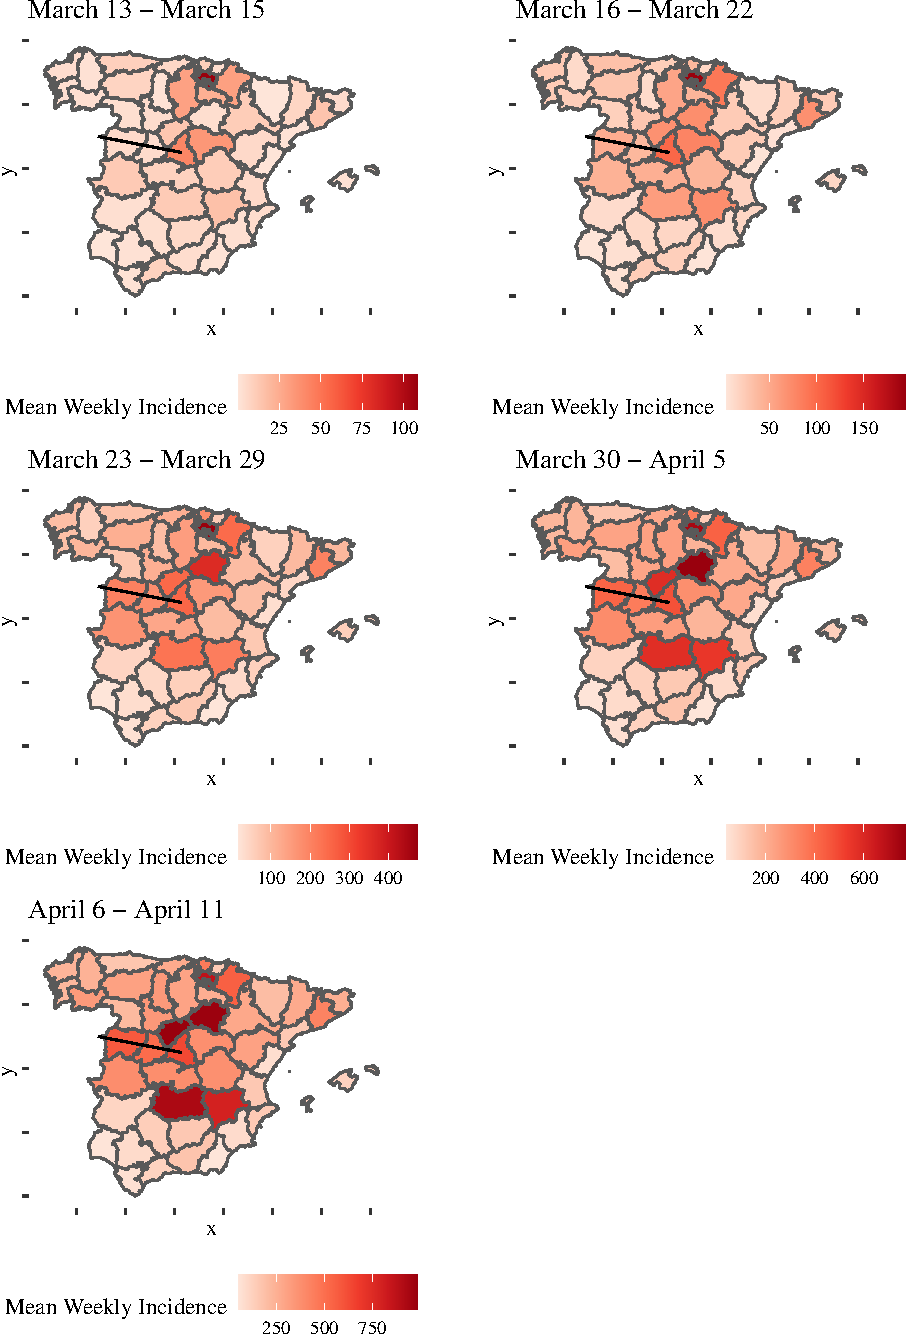
\includegraphics{Environmental-Correlates-of-COVID19-Spain_files/figure-latex/weekly-average-incidence-map-1.pdf}
\caption{\label{fig:weekly-average-incidence-map}Mean weekly incidence
of COVID-19 by province, in reported cases by 100,000 people}
\end{figure}

To visualize the distribution of temperature and humidity we aggregate
the provinces by Autonomous Community. In Figure
\ref{fig:descriptives-temperature} the communities have been sorted by
latitude, so that Principado de Asturias is the northernmost community,
and Canarias the southernmost. There is a relatively wide range of
values both within and between provinces over the 30 day period
examined. The top panel of the figure shows the distribution of mean
temperature. The lowest mean temperature for a community on any given
day is 2.8C, and the highest is 22.4C for a range of approximately 20
degrees. Likewise, there is a great deal of variability in humidity, as
seen in the bottom panel of the figure, where the lowest mean humidity
for any community is 48.3 and the highest is 99.6. The actual values for
the provinces display somewhat more variability even.

\begin{figure}
\centering
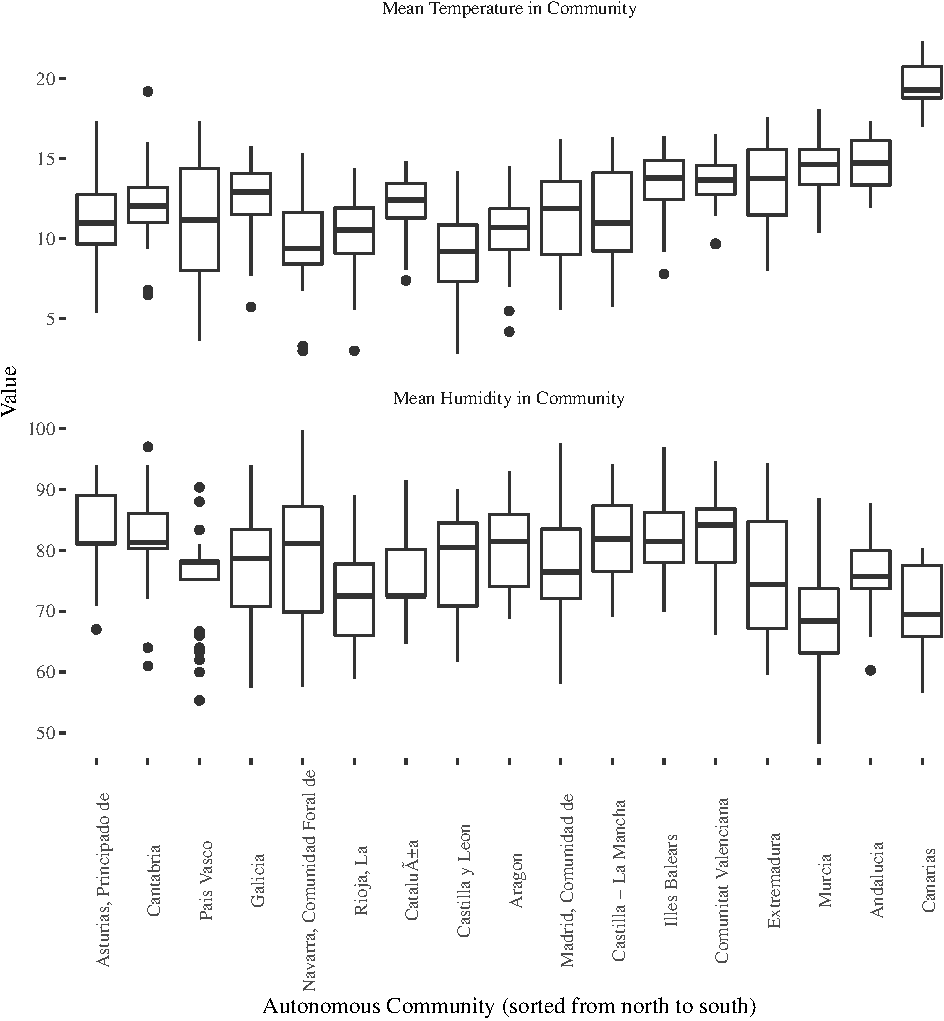
\includegraphics{Environmental-Correlates-of-COVID19-Spain_files/figure-latex/descriptives-temperature-1.pdf}
\caption{\label{fig:descriptives-temperature} Distribution of mean
temperatures and humidities in the Autonomous Communities in Spain
between March 12, 2020 and April 11, 2020. The Autonomous Communities
have been sorted by latitude, with communities to the left being the
northermost, and to the right the southernmost}
\end{figure}

\begin{figure}
\centering
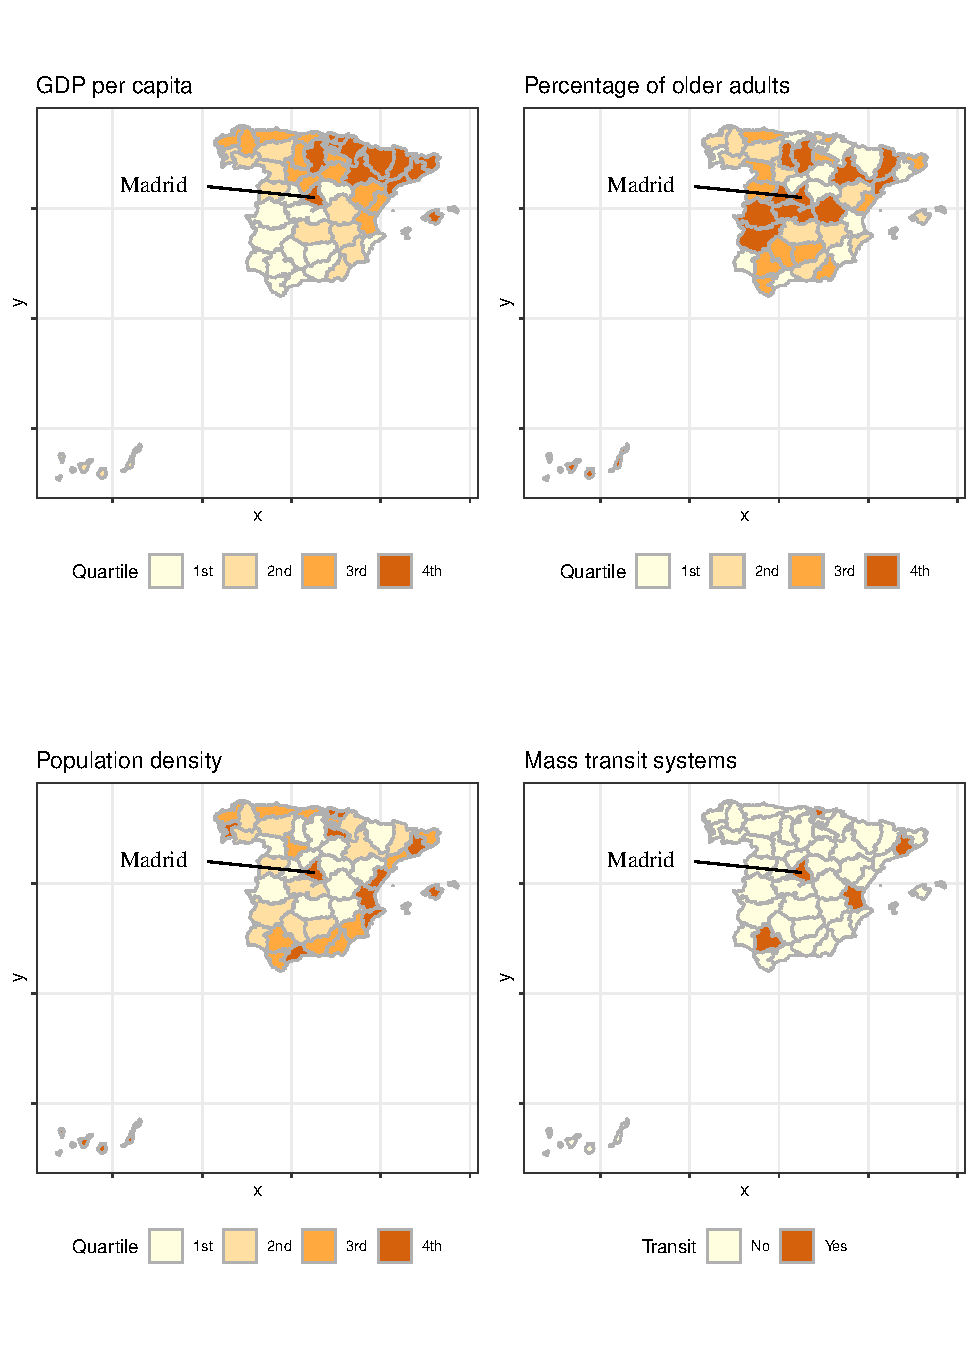
\includegraphics{Environmental-Correlates-of-COVID19-Spain_files/figure-latex/map-controls-1.pdf}
\caption{\label{fig:map-controls}Spatial distribution of control
variables by province}
\end{figure}

Figure \ref{fig:daily-correlations} shows the distribution of daily
correlations of the independent variables with incidence of COVID-19,
after log-transforming all variables. It can be seen there that the
correlation of GDPpc and temperature (in its three definitions) have the
strongest positive and negative correlations with incidence,
respectively. Percentage of older adults displays somewhat weaker
negative correlations with incidence, as does density. It can be seen
that the humidity variable, in its three forms, tends to be possitively
correlated with incidence of COVID-19.

\begin{figure}
\centering
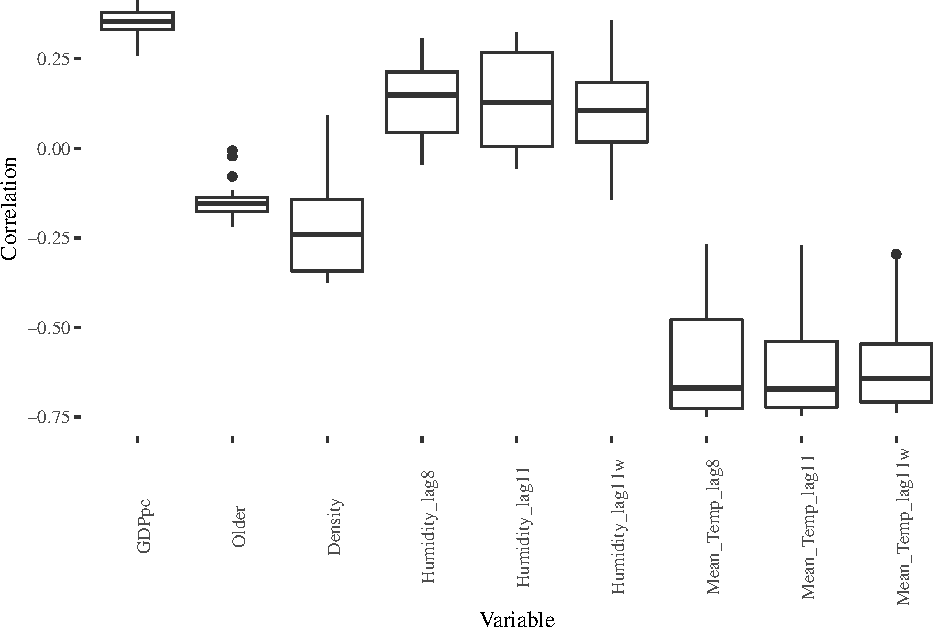
\includegraphics{Environmental-Correlates-of-COVID19-Spain_files/figure-latex/daily-correlations-1.pdf}
\caption{\label{fig:daily-correlations}Distribution of daily
correlations of the independent variables with daily incidence of
COVID-19 (all variables have been log-transformed)}
\end{figure}

\hypertarget{sur-models}{%
\subsection{SUR Models}\label{sur-models}}

The goodness of fit of the three systems of equations is shown in Figure
\ref{fig:goodness-of-fit}.

\begin{figure}
\centering
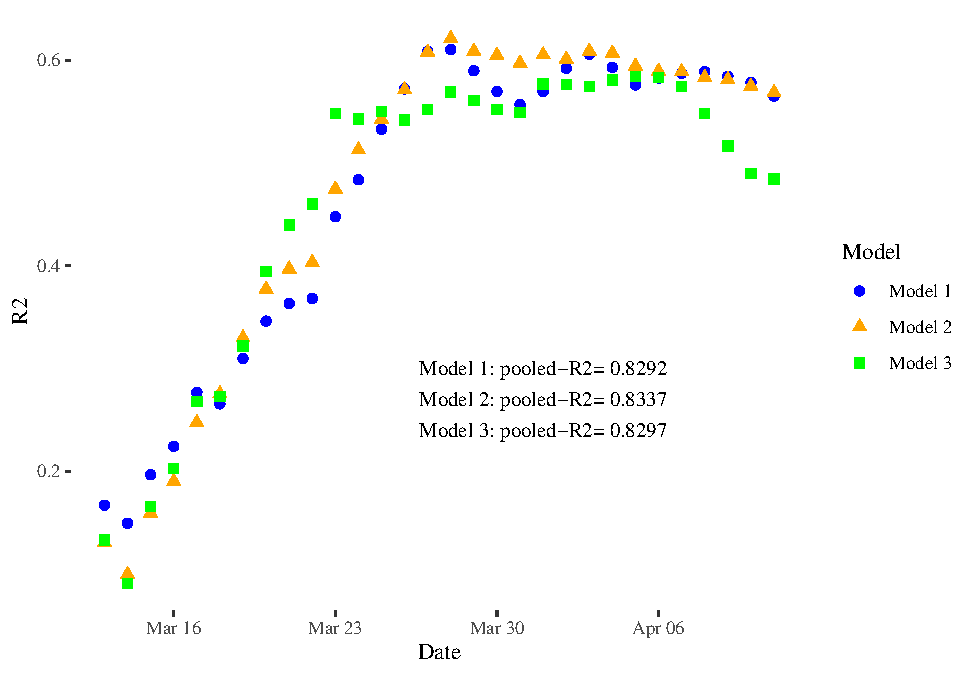
\includegraphics{Environmental-Correlates-of-COVID19-Spain_files/figure-latex/goodness-of-fit-1.pdf}
\caption{\label{fig:goodness-of-fit} Goodness of fit of the SUR systems:
by date and pooled}
\end{figure}

Summary of best model.

\begin{table}

\caption{\label{tab:summary-best-model}\label{tab:summary-best-model}Summary of estimation results best model (lagged 11-day moving average)}
\centering
\resizebox{\linewidth}{!}{
\begin{tabular}[t]{lrrrrrrl}
\toprule
\multicolumn{1}{c}{ } & \multicolumn{3}{c}{Estimates} & \multicolumn{3}{c}{Significance} & \multicolumn{1}{c}{ } \\
\cmidrule(l{3pt}r{3pt}){2-4} \cmidrule(l{3pt}r{3pt}){5-7}
Variable & Min & Mean & Max & p > 0.10 & 0.10 <= p < 0.05 & p <= 0.05 & Note\\
\midrule
\rowcolor{gray!6}  Intercept & 7.370 & 10.037 & 12.968 & 0 & 0 & 30 & Non-constrained\\
log(GDPpc) & 0.620 & 0.620 & 0.620 & 0 & 0 & 1 & Constrained\\
\rowcolor{gray!6}  log(Older) & -0.737 & -0.737 & -0.737 & 0 & 0 & 1 & Constrained\\
log(Density) & -0.220 & -0.097 & 0.153 & 19 & 1 & 10 & Non-constrained\\
\rowcolor{gray!6}  Transit & 0.314 & 0.512 & 0.583 & 10 & 9 & 11 & Non-constrained\\
\addlinespace
log(Humidity) & -1.434 & -0.534 & -0.031 & 10 & 1 & 19 & Non-constrained\\
\rowcolor{gray!6}  log(Temperature) & -2.014 & -1.406 & -0.929 & 0 & 0 & 30 & Non-constrained\\
log(Sunshine) & -0.258 & 0.097 & 0.206 & 7 & 2 & 21 & Non-constrained\\
\bottomrule
\multicolumn{8}{l}{\textit{Note: }}\\
\multicolumn{8}{l}{Significance: This is the number of coefficients with p-values as indicated}\\
\multicolumn{8}{l}{Non-constrained: coefficient was allowed to vary across equations}\\
\multicolumn{8}{l}{Constrained: coefficient as constant across equations}\\
\end{tabular}}
\end{table}

\hypertarget{discussion}{%
\section{Discussion}\label{discussion}}

Figure \ref{fig:delta-time} shows the temporal evolution of the spatial
autocorrelation coefficient (\(\lambda\)).

\begin{figure}
\centering
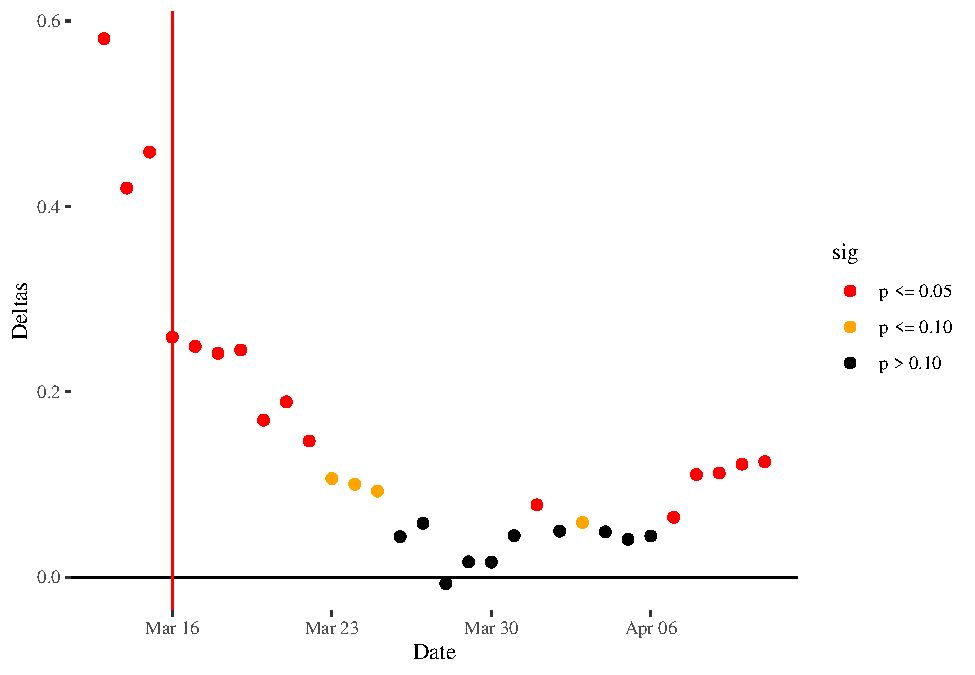
\includegraphics{Environmental-Correlates-of-COVID19-Spain_files/figure-latex/delta-time-1.pdf}
\caption{\label{fig:delta-time}Temporal evolution of the spatial
autocorrelation coefficient; dots are the point estimates and vertical
lines are 95\% confidence intervals. In yellow is the period after the
declaration of the state of emergency, and in orange is the period when
only essential activities were allowed.}
\end{figure}

Figure \ref{fig:beta-intercept-time} shows the temporal evolution of the
intercept.

\begin{figure}
\centering
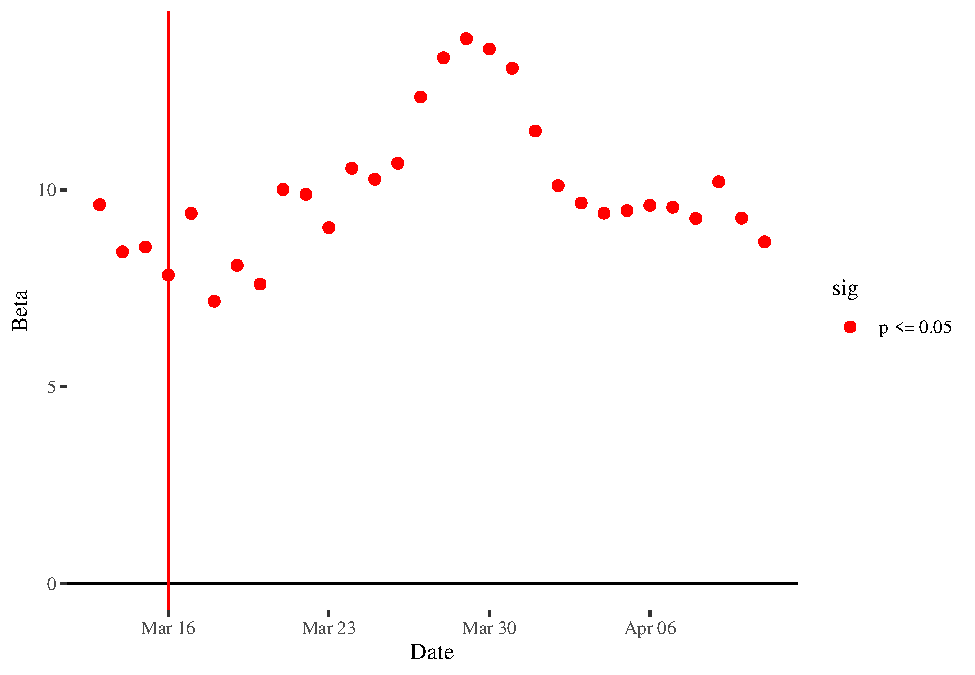
\includegraphics{Environmental-Correlates-of-COVID19-Spain_files/figure-latex/beta-intercept-time-1.pdf}
\caption{\label{fig:beta-intercept-time}Temporal evolution of intercept;
dots are the point estimates and vertical lines are 95\% confidence
intervals. In yellow is the period after the declaration of the state of
emergency, and in orange is the period when only essential activities
were allowed.}
\end{figure}

Figure \ref{fig:beta-density-time} shows the temporal evolution of the
coefficient for \(\log(Density)\).

\begin{figure}
\centering
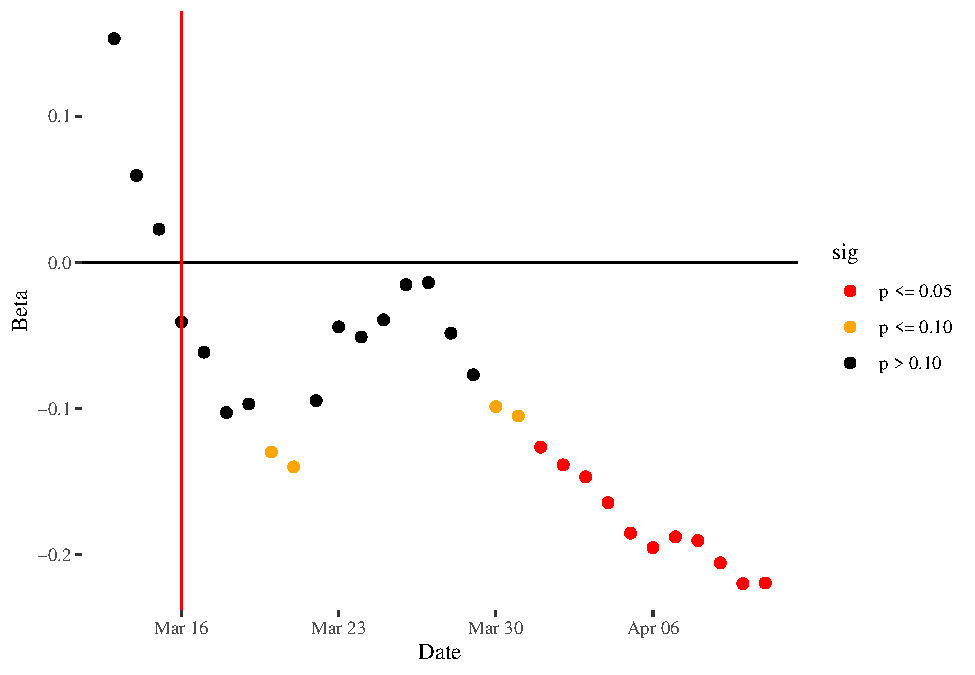
\includegraphics{Environmental-Correlates-of-COVID19-Spain_files/figure-latex/beta-density-time-1.pdf}
\caption{\label{fig:beta-density-time}Temporal evolution of coefficient
for log(Density); dots are the point estimates and vertical lines are
95\% confidence intervals. In yellow is the period after the declaration
of the state of emergency, and in orange is the period when only
essential activities were allowed.}
\end{figure}

Figure \ref{fig:beta-transit-time} shows the temporal evolution of the
coefficient for \(Transit\).

\begin{figure}
\centering
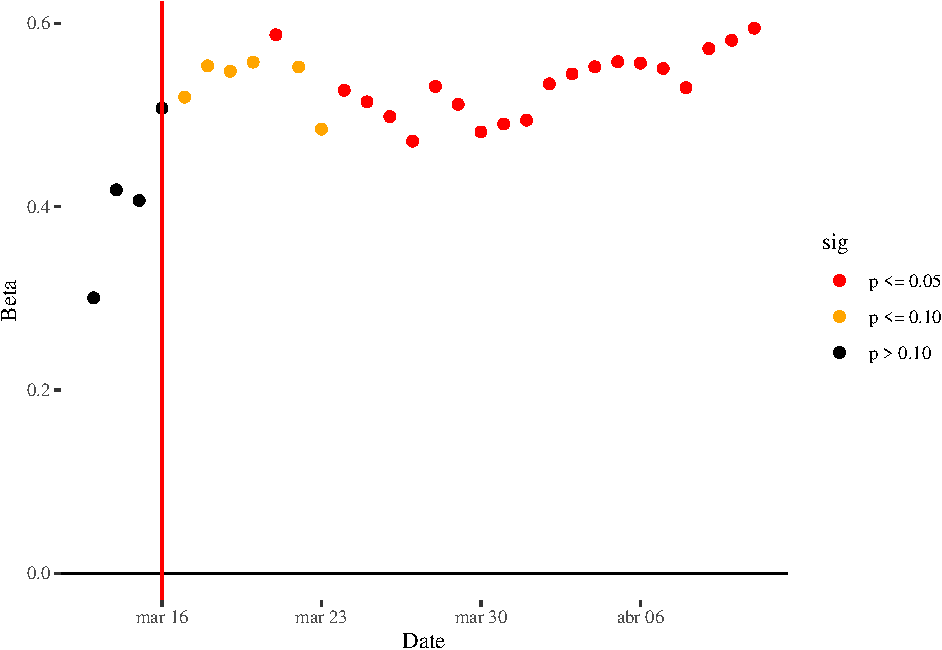
\includegraphics{Environmental-Correlates-of-COVID19-Spain_files/figure-latex/beta-transit-time-1.pdf}
\caption{\label{fig:beta-transit-time}Temporal evolution of coefficient
for Transit; dots are the point estimates and vertical lines are 95\%
confidence intervals. In yellow is the period after the declaration of
the state of emergency, and in orange is the period when only essential
activities were allowed.}
\end{figure}

Figure \ref{fig:beta-humidity-time} shows the temporal evolution of the
coefficient for \(\log(Humidity)\).

\begin{figure}
\centering
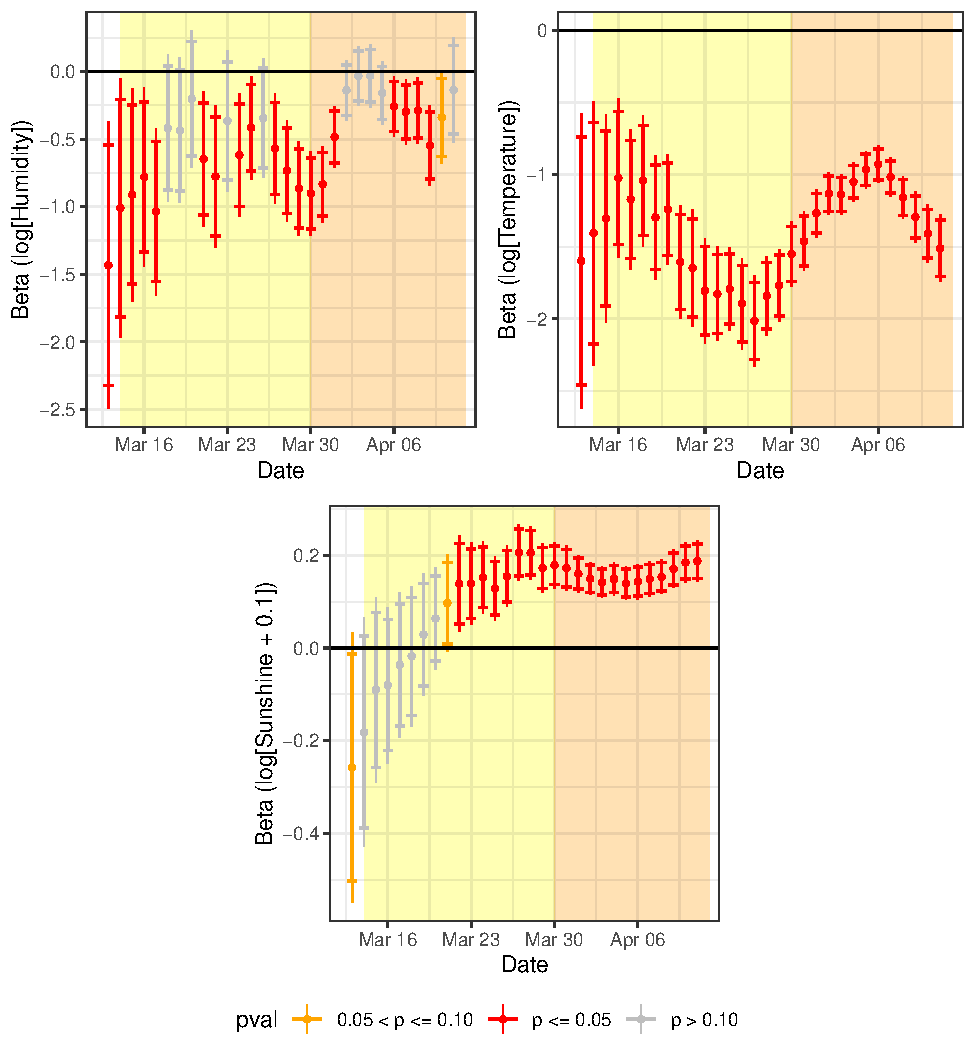
\includegraphics{Environmental-Correlates-of-COVID19-Spain_files/figure-latex/beta-humidity-time-1.pdf}
\caption{\label{fig:beta-humidity-time}Temporal evolution of coefficient
for log(Humidity); dots are the point estimates and vertical lines are
95\% confidence intervals. In yellow is the period after the declaration
of the state of emergency, and in orange is the period when only
essential activities were allowed.}
\end{figure}

Figure \ref{fig:beta-temperature-time} shows the temporal evolution of
the coefficient for \(\log(Temperature)\).

\begin{figure}
\centering
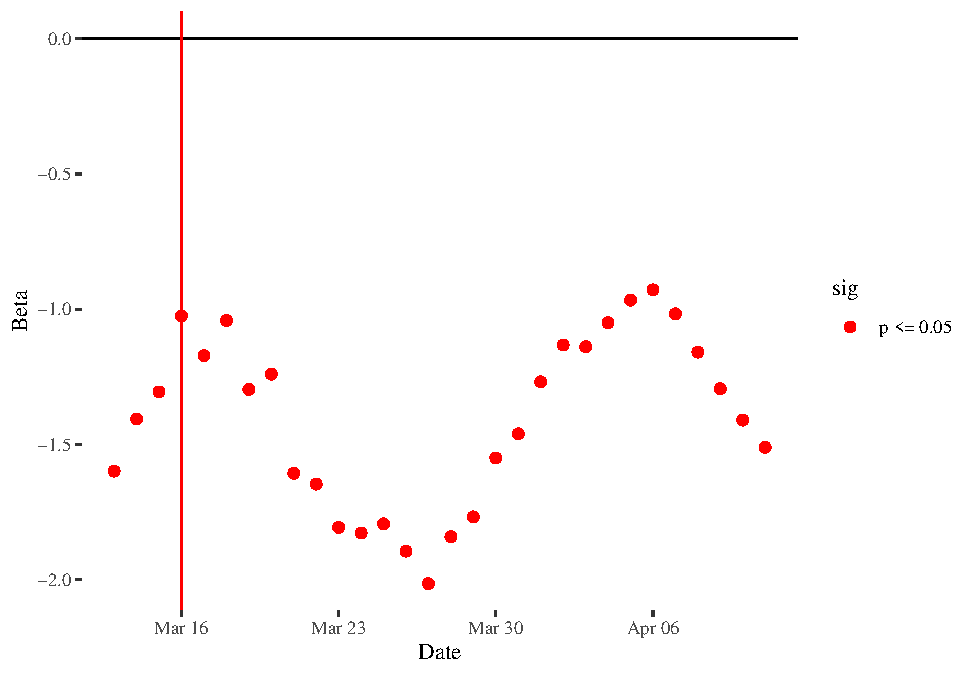
\includegraphics{Environmental-Correlates-of-COVID19-Spain_files/figure-latex/beta-temperature-time-1.pdf}
\caption{\label{fig:beta-temperature-time}Temporal evolution of
coefficient for log(Temperature); dots are the point estimates and
vertical lines are 95\% confidence intervals. In yellow is the period
after the declaration of the state of emergency, and in orange is the
period when only essential activities were allowed.}
\end{figure}

Figure \ref{fig:beta-sunshine-time} shows the temporal evolution of the
coefficient for \(\log(Sunshine + 0.1)\).

\begin{figure}
\centering
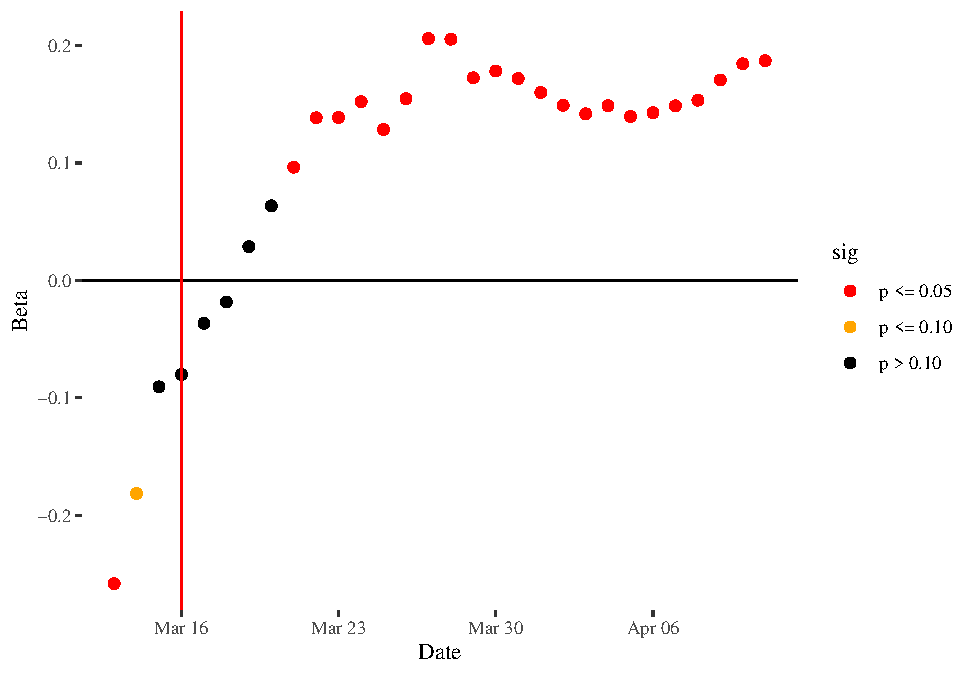
\includegraphics{Environmental-Correlates-of-COVID19-Spain_files/figure-latex/beta-sunshine-time-1.pdf}
\caption{\label{fig:beta-sunshine-time}Temporal evolution of coefficient
for log(Sunshine + 0.1); dots are the point estimates and vertical lines
are 95\% confidence intervals. In yellow is the period after the
declaration of the state of emergency, and in orange is the period when
only essential activities were allowed.}
\end{figure}

\hypertarget{concluding-remarks}{%
\section{Concluding Remarks}\label{concluding-remarks}}

More words go here.

Limitaciones

\begin{itemize}
\item
  La temperatura puedes ser un factor pero cabría esperar que no tuviera
  un impacto lineal. Por el contrario deberiamos esperar un `punto de
  corte': Una temperatua mantenida superior a X grados durante siete
  días sea la mejor forma de incorporarla al modelo. En nuestro modelo
  (log-log) en incremento en un 1\% de la temperatura se asocia con un
  incremento beta\% en la incidencia. Esto es lo mismo si la temperatura
  es baja que si es alta.
\item
  Idem para la humedad y horas de sol
\item
  Los datos son `provisionales'. Hay gran confusión sobre la incidencia
  real. La ausencia de test de diagnóstico PCRs al inicio de la pandemia
  (también ahora) puede desvirtuar el número de casos dianosticados.
\item
  Los datos oficiales (que tampoco son fiables) son reportados a nivel
  de Comunidades Autónomas. La recopilación de datos a nivel de
  provincial son el resultado de un esfuerzo colaborativo de
  recopilacion entre distintas fuentes (principalmente gobiernos
  locales). Nuevamente puede haber sesgos importanes.
\item
  En carácter insular de las Islas Canarias y de las Islas baleares no
  se ha tenido en cuenta.
\item
  Baleares se ha linkado artificialmente con 3/4 provincias y debería de
  haberse dejado aislada para respetar su carácter insular al definir la
  matriz W.
\item
  La incidencia depende de un estado inicial. Al inicio del estudio
  había provincias en las que la epidemia estaba muy desarrollada
  (Madrid/Alava) mientras que en otras apenas habías casos. Este hecho
  no ha sido considerado en el modelo. Decretar el confinamiento debe
  tener distintos impactos entre provincias. QUIZAR METER UNA VARAIBLE
  DUMMY CON COEF BETA CONSTANTE PARA CONTROLAR AQUELLAS PROVINCIAS CON
  MAYOR NUEMRO DE CASOS AL INICIO DEL CONFINAMIENTO.
\item
  No se ha controlado por el sistema sanitario de cada provincia. Uno de
  los principales focos de contagio han sido los hospitales y los
  centros de salud. En aquellas provincias donde se ha promovido el
  mensaje ``NO IR AL MEDICO'' han presentado menor incidencia.
\item
  HAY QUE INCLUIR INTERVALOS DE CONFIANZA EN LOS GRÁFICOS QUE HACEMOS DE
  LOS COEFICIENTES DEL MODELO
\item
  ¿hasta que punto las variables de control no recojen también factores
  climáticos? por ejemplo, la gente jóven vive en el sur de España que
  ha tenido menos incidencia.
\item
  TITULO: A spatial analysis of the environmental correlates ofCOVID-19
  incidence in Spain ¿during the lookdown?
\item
  Las estaciones meteorológicas para la obtencion de datos climáticos
  has sido elegidas aleatoriamente (una para cada provincia). otra
  seleccion puede dar otros resultados. AQUI SE PODRÍA HACER EL ESFUERZO
  DE CONSIDERARLAS TODAS (1000) Y CALCULAR LA MEDIA DE LAS VARAIBLES POR
  PROVINCIA
\end{itemize}

*IDEM para la humedad. idem para sunshine

\begin{itemize}
\tightlist
\item
  HACE FALTA INCLUIR UN PLOT CON LAS CORRELACIONES DE LOS RESIDUOS PARA
  DARLE RELEVANCIA A LA ESTIMACION SUR
\end{itemize}

\hypertarget{acknowledgments}{%
\section*{Acknowledgments}\label{acknowledgments}}
\addcontentsline{toc}{section}{Acknowledgments}

Add acknowledgments as appropriate in final draft.

The following \texttt{R} packages were used in the course of this
investigation and the authors wish to acknowledge their developers:
\texttt{aemet} {[}{]}, \texttt{ggthemes} (Arnold, 2019),
\texttt{gridExtra} (Auguie, 2017), \texttt{kableExtra} (Zhu, 2019),
\texttt{knitr} (Xie, 2015, 2014), \texttt{lubridate} (Grolemund and
Wickham, 2011), \texttt{plm} (Millo, 2017), \texttt{rticles} (Allaire et
al., 2020), \texttt{sf} (Pebesma, 2018), \texttt{spdep} (Bivand et al.,
2013), spsur (Angulo et al., 2020) \texttt{tidyverse} (Wickham et al.,
2019), \texttt{units} (Pebesma et al., 2016).

\hypertarget{references}{%
\section*{References}\label{references}}
\addcontentsline{toc}{section}{References}

\hypertarget{refs}{}
\leavevmode\hypertarget{ref-Allaire2020}{}%
Allaire, J., Xie, Y., R Foundation, Wickham, H., Journal of Statistical
Software, Vaidyanathan, R., Association for Computing Machinery,
Boettiger, C., Elsevier, Broman, K., Mueller, K., Quast, B., Pruim, R.,
Marwick, B., Wickham, C., Keyes, O., Yu, M., Emaasit, D., Onkelinx, T.,
Gasparini, A., Desautels, M.-A., Leutnant, D., MDPI, Taylor and Francis,
Ögreden, O., Hance, D., Nüst, D., Uvesten, P., Campitelli, E.,
Muschelli, J., Kamvar, Z.N., Ross, N., Cannoodt, R., Luguern, D.,
Kaplan, D.M., 2020. Rticles: Article formats for r markdown.

\leavevmode\hypertarget{ref-Angulo2020spsur}{}%
Angulo, A., Lopez, F.A., Minguez, R., Mur, J., 2020. Spsur: Spatial
seemingly unrelated regression models.

\leavevmode\hypertarget{ref-Anselin1988spatial}{}%
Anselin, L., 1988. Spatial econometrics: Methods and models, Studies in
operational regional science. Kluwer Academic Publishers, Dordrecht.

\leavevmode\hypertarget{ref-Anselin2016estimation}{}%
Anselin, L., 2016. Estimation and testing in the spatial seemingly
unrelated regression (sur). Geoda Center for Geospatial Analysis;
Computation, Arizona State University. Working Paper 2016-01.

\leavevmode\hypertarget{ref-Araujo2020spread}{}%
Araujo, M.B., Naimi, B., 2020. Spread of sars-cov-2 coronavirus likely
to be constrained by climate. medRxiv.

\leavevmode\hypertarget{ref-Arnold2019}{}%
Arnold, J.B., 2019. Ggthemes: Extra themes, scales and geoms for
'ggplot2'.

\leavevmode\hypertarget{ref-Auguie2017gridextra}{}%
Auguie, B., 2017. GridExtra: Miscellaneous functions for "grid"
graphics.

\leavevmode\hypertarget{ref-deangel2020weathering}{}%
Ángel Solá, D.E. de, Wang, L., Vázquez, M., Lázaro, P.A.M., 2020.
Weathering the pandemic: How the caribbean basin can use viral and
environmental patterns to predict, prepare and respond to covid‐19.
Journal of Medical Virology.

\leavevmode\hypertarget{ref-Bivand2013}{}%
Bivand, R.S., Pebesma, E., Gomez-Rubio, V., 2013. Applied spatial data
analysis with R, second edition. Springer, NY.

\leavevmode\hypertarget{ref-Cao2010spatio}{}%
Cao, Z., Zeng, D., Zheng, X., Wang, Q., Wang, F., Wang, J., Wang, X.,
2010. Spatio-temporal evolution of beijing 2003 sars epidemic. Science
China Earth Sciences 53, 1017--1028.
doi:\href{https://doi.org/10.1007/s11430-010-0043-x}{10.1007/s11430-010-0043-x}

\leavevmode\hypertarget{ref-Casanova2010effects}{}%
Casanova, L.M., Jeon, S., Rutala, W.A., Weber, D.J., Sobsey, M.D., 2010.
Effects of air temperature and relative humidity on coronavirus survival
on surfaces. Appl. Environ. Microbiol. 76, 2712--2717.

\leavevmode\hypertarget{ref-Chan2011effects}{}%
Chan, K., Peiris, J., Lam, S., Poon, L., Yuen, K., Seto, W., 2011. The
effects of temperature and relative humidity on the viability of the
sars coronavirus. Advances in virology 2011.

\leavevmode\hypertarget{ref-Cliff1998detecting}{}%
Cliff, A., Haggett, P., Smallman-Raynor, M., 1998. Detecting
space---time patterns in geocoded disease data. Cholera in london, 1854
measles in the united states, 1962--95, in: Geomed'97. Springer, pp.
13--42.

\leavevmode\hypertarget{ref-Coelho2020exponential}{}%
Coelho, M.T.P., Rodrigues, J.F.M., Medina, A.M., Scalco, P., Terribile,
L.C., Vilela, B., Diniz-Filho, J.A.F., Dobrovolski, R., 2020.
Exponential phase of covid19 expansion is not driven by climate at
global scale. medRxiv.

\leavevmode\hypertarget{ref-Desjardins2020rapid}{}%
Desjardins, M., Hohl, A., Delmelle, E., 2020. Rapid surveillance of
covid-19 in the united states using a prospective space-time scan
statistic: Detecting and evaluating emerging clusters. Applied Geography
102202.

\leavevmode\hypertarget{ref-Fernandes2020economic}{}%
Fernandes, N., 2020. Economic effects of coronavirus outbreak (covid-19)
on the world economy. Available at SSRN 3557504.

\leavevmode\hypertarget{ref-Gong2020balance}{}%
Gong, B., Zhang, S., Yuan, L., Chen, K.Z., 2020. A balance act:
Minimizing economic loss while controlling novel coronavirus pneumonia.
Journal of Chinese Governance 1--20.

\leavevmode\hypertarget{ref-Greene2003econometric}{}%
Greene, W.H., 2003. Econometric analysis. Pearson Education India.

\leavevmode\hypertarget{ref-Grolemund2011dates}{}%
Grolemund, G., Wickham, H., 2011. Dates and times made easy with
lubridate. Journal of Statistical Software 40, 1--25.

\leavevmode\hypertarget{ref-Hallet2002regional}{}%
Hallet, M., 2002. Regional specialisation and concentration in the eu,
in: Regional Convergence in the European Union. Springer, pp. 53--76.

\leavevmode\hypertarget{ref-Harbert2020spatial}{}%
Harbert, R.S., Cunningham, S.W., Tessler, M., 2020. Spatial modeling
cannot currently differentiate sars-cov-2 coronavirus and human
distributions on the basis of climate in the united states. medRxiv.

\leavevmode\hypertarget{ref-Hu2013scaling}{}%
Hu, H., Nigmatulina, K., Eckhoff, P., 2013. The scaling of contact rates
with population density for the infectious disease models. Mathematical
Biosciences 244, 125--134.
doi:\href{https://doi.org/https://doi.org/10.1016/j.mbs.2013.04.013}{https://doi.org/10.1016/j.mbs.2013.04.013}

\leavevmode\hypertarget{ref-Jaakkola2014decline}{}%
Jaakkola, K., Saukkoriipi, A., Jokelainen, J., Juvonen, R., Kauppila,
J., Vainio, O., Ziegler, T., Rönkkö, E., Jaakkola, J.J., Ikäheimo, T.M.,
2014. Decline in temperature and humidity increases the occurrence of
influenza in cold climate. Environmental Health 13, 22.

\leavevmode\hypertarget{ref-Jones2008global}{}%
Jones, K.E., Patel, N.G., Levy, M.A., Storeygard, A., Balk, D.,
Gittleman, J.L., Daszak, P., 2008. Global trends in emerging infectious
diseases. Nature 451, 990--993.
doi:\href{https://doi.org/10.1038/nature06536}{10.1038/nature06536}

\leavevmode\hypertarget{ref-Kissler2020projecting}{}%
Kissler, S.M., Tedijanto, C., Goldstein, E., Grad, Y.H., Lipsitch, M.,
2020. Projecting the transmission dynamics of sars-cov-2 through the
postpandemic period. Science eabb5793.
doi:\href{https://doi.org/10.1126/science.abb5793}{10.1126/science.abb5793}

\leavevmode\hypertarget{ref-Kudo2019low}{}%
Kudo, E., Song, E., Yockey, L.J., Rakib, T., Wong, P.W., Homer, R.J.,
Iwasaki, A., 2019. Low ambient humidity impairs barrier function and
innate resistance against influenza infection. Proceedings of the
National Academy of Sciences 116, 10905--10910.

\leavevmode\hypertarget{ref-Lancastle2020impact}{}%
Lancastle, N.M., 2020. Is the impact of social distancing on coronavirus
growth rates effective across different settings? A non-parametric and
local regression approach to test and compare the growth rate. medRxiv.

\leavevmode\hypertarget{ref-Lauer2020incubation}{}%
Lauer, S.A., Grantz, K.H., Bi, Q., Jones, F.K., Zheng, Q., Meredith,
H.R., Azman, A.S., Reich, N.G., Lessler, J., 2020. The incubation period
of coronavirus disease 2019 (covid-19) from publicly reported confirmed
cases: Estimation and application. Annals of Internal Medicine.
doi:\href{https://doi.org/10.7326/m20-0504}{10.7326/m20-0504}

\leavevmode\hypertarget{ref-Lauridsen2010spatiotemporal}{}%
Lauridsen, J., Bech, M., López, F., Maté, M., 2010. A spatiotemporal
analysis of public pharmaceutical expenditure. The Annals of Regional
Science 44, 299--314.

\leavevmode\hypertarget{ref-Legallo2006evaluating}{}%
Le Gallo, J., Dall'Erba, S., 2006. Evaluating the temporal and spatial
heterogeneity of the european convergence process, 1980--1999. Journal
of Regional Science 46, 269--288.

\leavevmode\hypertarget{ref-Lopez2017spatial}{}%
López, F.A., Martínez-Ortiz, P.J., Cegarra-Navarro, J.-G., 2017. Spatial
spillovers in public expenditure on a municipal level in spain. The
Annals of Regional Science 58, 39--65.

\leavevmode\hypertarget{ref-Lopez2014spatial}{}%
López, F.A., Mur, J., Angulo, A., 2014. Spatial model selection
strategies in a sur framework. The case of regional productivity in eu.
The Annals of Regional Science 53, 197--220.

\leavevmode\hypertarget{ref-Luo2020how}{}%
Luo, S., Tsang, K.P., 2020. How much of china and world gdp has the
coronavirus reduced? Available at SSRN 3543760.

\leavevmode\hypertarget{ref-Makinen2009cold}{}%
Mäkainen, T.M., Juvonen, R., Jokelainen, J., Harju, T.H., Peitso, A.,
Bloigu, A., Silvennoinen-Kassinen, S., Leinonen, M., Hassi, J., 2009.
Cold temperature and low humidity are associated with increased
occurrence of respiratory tract infections. Respiratory medicine 103,
456--462.

\leavevmode\hypertarget{ref-Meijers2008strategic}{}%
Meijers, E., Hoekstra, J., Aguado, R., 2008. Strategic planning for city
networks: The emergence of a basque global city? International Planning
Studies 13, 239--259.
doi:\href{https://doi.org/10.1080/13563470802521440}{10.1080/13563470802521440}

\leavevmode\hypertarget{ref-Meng2005understanding}{}%
Meng, B., Wang, J., Liu, J., Wu, J., Zhong, E., 2005. Understanding the
spatial diffusion process of severe acute respiratory syndrome in
beijing. Public Health 119, 1080--1087.
doi:\href{https://doi.org/https://doi.org/10.1016/j.puhe.2005.02.003}{https://doi.org/10.1016/j.puhe.2005.02.003}

\leavevmode\hypertarget{ref-Millo2017robust}{}%
Millo, G., 2017. Robust standard error estimators for panel models: A
unifying approach. Journal of Statistical Software 82, 1--27.
doi:\href{https://doi.org/10.18637/jss.v082.i03}{10.18637/jss.v082.i03}

\leavevmode\hypertarget{ref-Minguez2019}{}%
Mínguez, R., López, F., Mur, J., 2019. ML versus iv estimates of spatial
sur models: Evidence from the case of airbnb in madrid urban area. The
Annals of Regional Science 1--35.

\leavevmode\hypertarget{ref-Morency2011distance}{}%
Morency, C., Páez, A., Roorda, M.J., Mercado, R.G., Farber, S., 2011.
Distance traveled in three canadian cities: Spatial analysis from the
perspective of vulnerable population segments. Journal of Transport
Geography 19, 39--50.

\leavevmode\hypertarget{ref-National2020rapid}{}%
National Academies of Sciences, Engineering and Medicine, 2020. Rapid
expert consultation on sars-cov-2 survival in relation to temperature
and humidity and potential for seasonality for the covid-19 pandemic
(april 7, 2020). The National Academies Press, Washington, DC.
doi:\href{https://doi.org/doi:10.17226/25771}{doi:10.17226/25771}

\leavevmode\hypertarget{ref-Pebesma2018}{}%
Pebesma, E., 2018. Simple Features for R: Standardized Support for
Spatial Vector Data. The R Journal 10, 439--446.
doi:\href{https://doi.org/10.32614/RJ-2018-009}{10.32614/RJ-2018-009}

\leavevmode\hypertarget{ref-Pebesma2016}{}%
Pebesma, E., Mailund, T., Hiebert, J., 2016. Measurement units in R. R
Journal 8, 486--494.
doi:\href{https://doi.org/10.32614/RJ-2016-061}{10.32614/RJ-2016-061}

\leavevmode\hypertarget{ref-Perez2009agent}{}%
Perez, L., Dragicevic, S., 2009. An agent-based approach for modeling
dynamics of contagious disease spread. International journal of health
geographics 8, 50.

\leavevmode\hypertarget{ref-Prem2017projecting}{}%
Prem, K., Cook, A.R., Jit, M., 2017. Projecting social contact matrices
in 152 countries using contact surveys and demographic data. PLoS
computational biology 13, e1005697.

\leavevmode\hypertarget{ref-Rey1999us}{}%
Rey, S.J., Montouri, B.D., 1999. US regional income convergence: A
spatial econometric perspective. Regional studies 33, 143--156.

\leavevmode\hypertarget{ref-Roorda2010trip}{}%
Roorda, M.J., Paez, A., Morency, C., Mercado, R., Farber, S., 2010. Trip
generation of vulnerable populations in three canadian cities: A spatial
ordered probit approach. Transportation 37, 525--548.
doi:\href{https://doi.org/10.1007/s11116-010-9263-3}{10.1007/s11116-010-9263-3}

\leavevmode\hypertarget{ref-Sikder2012immobility}{}%
Sikder, S., Pinjari, A.R., 2012. Immobility levels and mobility
preferences of the elderly in the united states evidence from 2009
national household travel survey. Transportation Research Record
137--147. doi:\href{https://doi.org/10.3141/2318-16}{10.3141/2318-16}

\leavevmode\hypertarget{ref-Singh2020age}{}%
Singh, R., Adhikari, R., 2020. Age-structured impact of social
distancing on the covid-19 epidemic in india. arXiv preprint
arXiv:2003.12055.

\leavevmode\hypertarget{ref-Novel2020epidemiological}{}%
The Novel Coronavirus Pneumonia Emergency Response Epidemiology Team,
2020. The epidemiological characteristics of an outbreak of 2019 novel
coronavirus diseases (covid-19)---china, 2020. China CDC Weekly 2,
113--122.

\leavevmode\hypertarget{ref-vanWagner2008toward}{}%
Van Wagner, E., 2008. Toward a dialectical understanding of networked
disease in the global city: Vulnerability, connectivity, topologies.
Networked disease: Emerging infections in the global city 13--26.

\leavevmode\hypertarget{ref-Wang2010gis}{}%
Wang, J., Xiong, J., Yang, K., Peng, S., Xu, Q., 2010. Use of gis and
agent-based modeling to simulate the spread of influenza, in: 2010 18th
International Conference on Geoinformatics. IEEE, pp. 1--6.

\leavevmode\hypertarget{ref-Wickham2019}{}%
Wickham, H., Averick, M., Bryan, J., Chang, W., McGowan, L.D., François,
R., Grolemund, G., Hayes, A., Henry, L., Hester, J., Kuhn, M., Pedersen,
T.L., Miller, E., Bache, S.M., Müller, K., Ooms, J., Robinson, D.,
Seidel, D.P., Spinu, V., Takahashi, K., Vaughan, D., Wilke, C., Woo, K.,
Yutani, H., 2019. Welcome to the tidyverse. Journal of Open Source
Software 4, 1686.
doi:\href{https://doi.org/10.21105/joss.01686}{10.21105/joss.01686}

\leavevmode\hypertarget{ref-Xie2014}{}%
Xie, Y., 2014. Knitr: A comprehensive tool for reproducible research in
R, in: Stodden, V., Leisch, F., Peng, R.D. (Eds.), Implementing
Reproducible Computational Research. Chapman; Hall/CRC.

\leavevmode\hypertarget{ref-Xie2015}{}%
Xie, Y., 2015. Dynamic documents with R and knitr, 2nd ed. Chapman;
Hall/CRC, Boca Raton, Florida.

\leavevmode\hypertarget{ref-Yao2020association}{}%
Yao, Y., Pan, J., Liu, Z., Meng, X., Wang, W., Kan, H., Wang, W., 2020.
No association of covid-19 transmission with temperature or uv radiation
in chinese cities. European Respiratory Journal 2000517.
doi:\href{https://doi.org/10.1183/13993003.00517-2020}{10.1183/13993003.00517-2020}

\leavevmode\hypertarget{ref-Zellner1962efficient}{}%
Zellner, A., 1962. An efficient method of estimating seemingly unrelated
regressions and tests for aggregation bias. Journal of the American
statistical Association 57, 348--368.

\leavevmode\hypertarget{ref-Zhou2016accelerated}{}%
Zhou, Y.R., Coleman, W.D., 2016. Accelerated contagion and response:
Understanding the relationships among globalization, time, and disease.
Globalizations 13, 285--299.

\leavevmode\hypertarget{ref-Zhu2019}{}%
Zhu, H., 2019. KableExtra: Construct complex table with 'kable' and pipe
syntax.


\end{document}


